\documentclass{article}
\usepackage{geometry,amsmath,amssymb,graphicx,calc,ifthen,capt-of}
\geometry{letterpaper}

%%%%%%%%%% Start TeXmacs macros
\newcommand{\tmstrong}[1]{\textbf{#1}}
\newcommand{\tmtextit}[1]{{\itshape{#1}}}
\newenvironment{itemizeminus}{\begin{itemize} \renewcommand{\labelitemi}{$-$}\renewcommand{\labelitemii}{$-$}\renewcommand{\labelitemiii}{$-$}\renewcommand{\labelitemiv}{$-$}}{\end{itemize}}
\newcommand{\tmfloatcontents}{}
\newlength{\tmfloatwidth}
\newcommand{\tmfloat}[5]{
  \renewcommand{\tmfloatcontents}{#4}
  \setlength{\tmfloatwidth}{\widthof{\tmfloatcontents}+1in}
  \ifthenelse{\equal{#2}{small}}
    {\ifthenelse{\lengthtest{\tmfloatwidth > \linewidth}}
      {\setlength{\tmfloatwidth}{\linewidth}}{}}
    {\setlength{\tmfloatwidth}{\linewidth}}
  \begin{minipage}[#1]{\tmfloatwidth}
    \begin{center}
      \tmfloatcontents
      \captionof{#3}{#5}
    \end{center}
  \end{minipage}}
%%%%%%%%%% End TeXmacs macros

\setlength{\topmargin}{0in}
\setlength{\headheight}{0in}
\setlength{\headsep}{0in}
%\setlength{\textheight}{7.7in}
%\setlength{\textwidth}{6.5in}
\setlength{\oddsidemargin}{0in}
\setlength{\evensidemargin}{0in}
\setlength{\parindent}{0.0in}
\setlength{\parskip}{0.10in}

\begin{document}

\title{Converting Geomagnetic Field Vectors\\
to Earth Centered Inertial}\author{Matthew P. Wampler-Doty}\date{}\maketitle

This document details how to convert the geomagnetic field vectors output by
the NOAA World Magnetic Model (WMM) to an Earth Centered Inertial (ECI) frame.

Vectors in the WMM geomagnetic reference frame have three components:
\begin{itemizeminus}
  \item[$\widehat{\text{{\tmstrong{x}}}}$ --] the amplitude in the northerly
  direction
  
  \item[$\widehat{\text{{\tmstrong{y}}}}$ --] the amplitude in the easterly
  direction
  
  \item[$\widehat{\text{{\tmstrong{z}}}}$ --] the amplitude in the downward
  direction, towards the earth
\end{itemizeminus}
\begin{center}
  \tmfloat{h}{small}{figure}{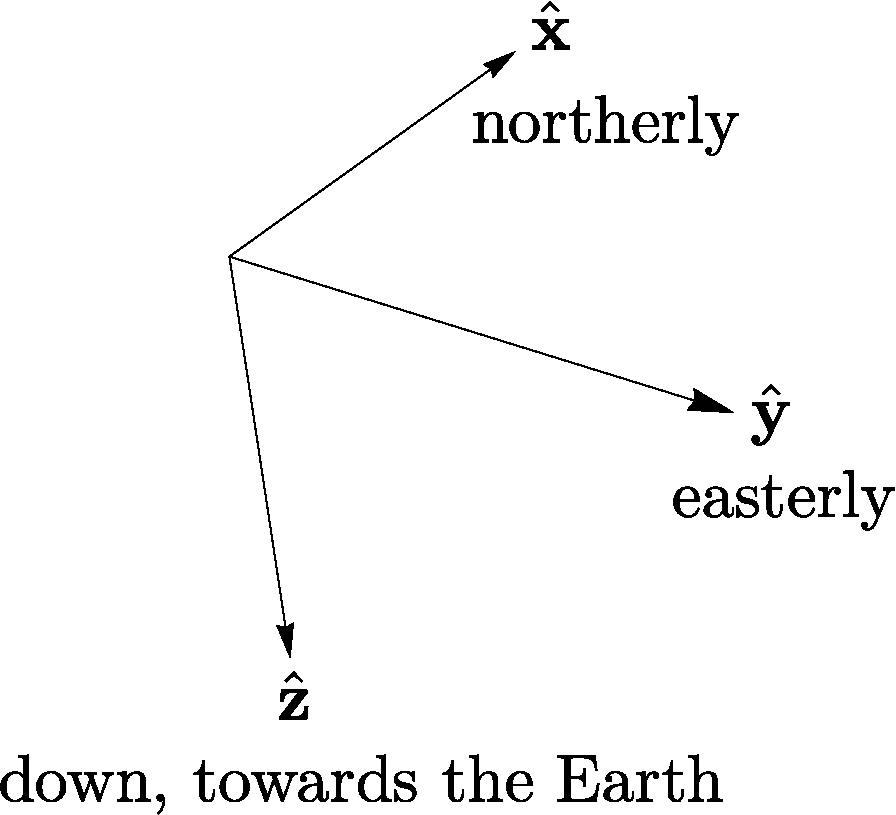
\includegraphics[scale=0.50]{geomag-ref-frame.pdf}}{The
  WMM geomagnetic reference frame}
\end{center}

Vectors in the ECI frame also have three components:
\begin{itemizeminus}
  \item[$\widehat{\text{{\tmstrong{v}}}}$ --] the amplitude in the direction of the
  vernal equinox
  
  \item[$\widehat{\text{{\tmstrong{u}}}}$ --] the amplitude in the direction of
  north of the ecliptic plane
  
  \item[$\widehat{\text{{\tmstrong{w}}}}$ --] the amplitude along the ecliptic
  plane that is orthogonal to the vernal equinox
\end{itemizeminus}
\begin{center}
  \tmfloat{h}{small}{figure}{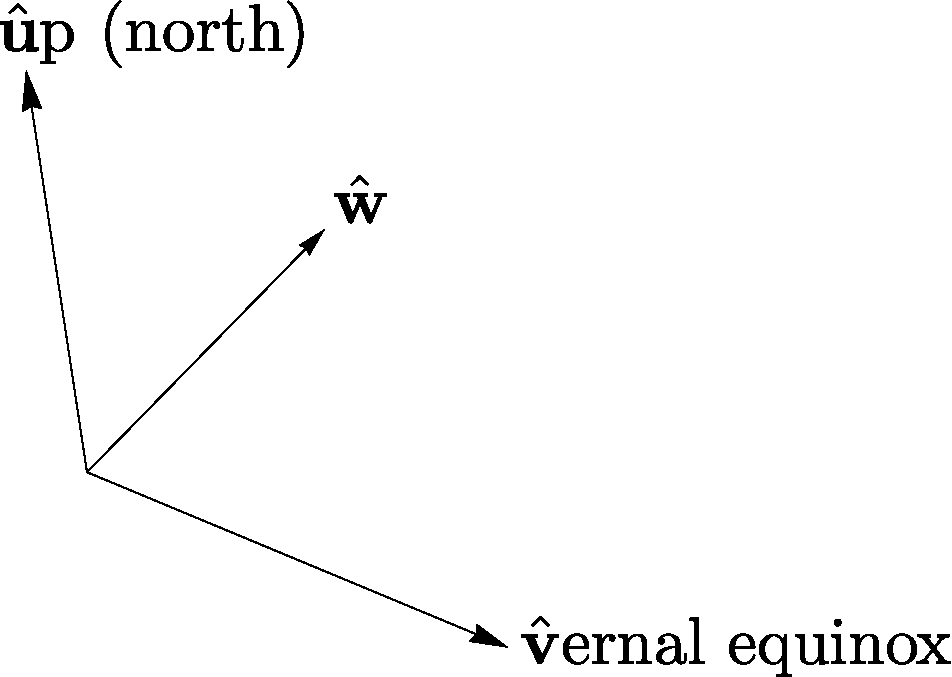
\includegraphics[scale=0.50]{eci-ref-frame.pdf}}{The
  ECI reference frame}
\end{center}

Both the WMM geomagnetic and ECI reference frames are right handed.



Every WMM geomagnetic field vector is associated with a latitude and longitude
at a particular time, which are in turn associated with a \tmtextit{right
ascension} $\rho$ and \tmtextit{declination} $\delta$ on the celestial sphere.



The coordinate transformations between WMM geomagnetic field vectors and ECI
vectors form two inverse rotations functional on $\rho$ and $\delta$, which we
represent as rotation matrices. \ It suffices to construct only one of these
transformations, since the inverse is given by the transpose.



We will illustrate how to translate an ECI vector into WMM geomagnetic vector.
\ Our motivation is depicted in Figure \ref{spherical-triangle}. \ This
depicts a spherical triangle on the earth, each corner representing certain
values for $\rho$ and $\delta$.

\begin{center}
  \tmfloat{h}{small}{figure}{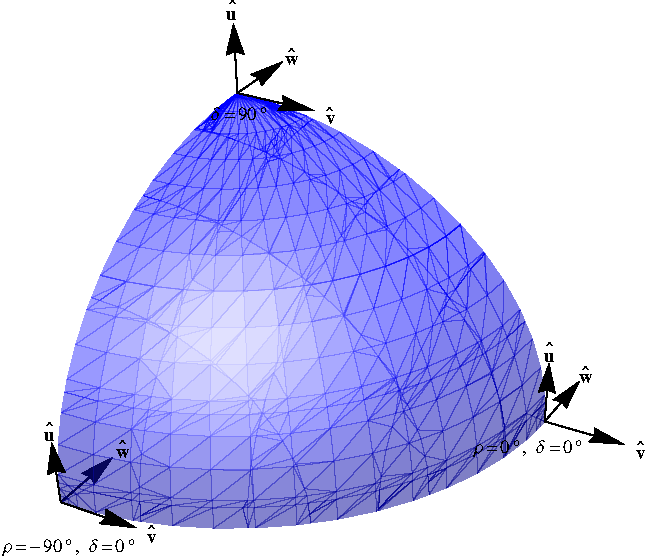
\includegraphics[scale=1]{spherical_triangle.pdf}}{\label{spherical-triangle}Spherical
  Triangle and ECI axes}
\end{center}

Using Figure \ref{spherical-triangle}, we can see how at different values of
$\rho$ and $\delta$ the ECI vector components translate into WMM magnetic
field vector components.

Take, for instance, the point where $\delta = 90^{\circ}$ (the north pole and
the top point in the diagram). \ We can see that
$\widehat{\text{{\tmstrong{z}}}} = - \text{$\widehat{\text{{\tmstrong{u}}}}$}$
at this point, that is the amplitude towards the earth of the geomagnetic
field vector is exactly the opposite of its amplitude north of the ecliptic. \
Likewise, we can see from the picture that for all points where $\delta =
0^{\circ}$, $\widehat{\text{{\tmstrong{z}}}}$ is orthogonal to
$\text{$\widehat{\text{{\tmstrong{u}}}}$}$. \ In fact the relationship is
\begin{equation}
  \widehat{\text{{\tmstrong{z}}}} \propto - \sin \delta
  \widehat{\text{{\tmstrong{u}}}} \label{eq1}
\end{equation}
By symmetry conditions, we know that $\pm \cos \delta$ must be split among the
other two unit vector components $\text{$\widehat{\text{{\tmstrong{v}}}}$}$
and $\text{$\widehat{\text{{\tmstrong{w}}}}$}$.

At the equator, where $\delta = 0^{\circ}$, we have drawn two other points to
consider. \ The first is where $\rho = 0^{\circ}$. \ At this point,
$\widehat{\text{{\tmstrong{z}}}} = -
\text{$\widehat{\text{{\tmstrong{v}}}}$}$. \ At $\rho = - 90^{\circ}$, we have
$\widehat{\text{{\tmstrong{z}}}} = \text{$\widehat{\text{{\tmstrong{w}}}}$}$.
\ Noting that both $\text{$\widehat{\text{{\tmstrong{v}}}}$}$ and
$\text{$\widehat{\text{{\tmstrong{w}}}}$}$ must split $\cos \delta$, we
observe the following other relationships:
\begin{equation}
  \widehat{\text{{\tmstrong{z}}}} \propto - \cos \delta \cos \rho
  \text{$\widehat{\text{{\tmstrong{v}}}}$} \label{eq2}
\end{equation}
\begin{equation}
  \widehat{\text{{\tmstrong{z}}}} \propto - \cos \delta \sin \rho
  \text{$\widehat{\text{{\tmstrong{w}}}}$} \label{eq3}
\end{equation}
Combining (\ref{eq1}), (\ref{eq2}), and (\ref{eq3}), we have:
\begin{equation}
  \widehat{\text{{\tmstrong{z}}}} = - \sin \delta
  \text{$\widehat{\text{{\tmstrong{u}}}}$} - \cos \delta \cos \rho
  \text{$\widehat{\text{{\tmstrong{v}}}}$} - \cos \delta \sin \rho
  \text{$\widehat{\text{{\tmstrong{w}}}}$} \label{eqz}
\end{equation}
One can take a dot product of the right hand side with itself and verify that
it is indeed 1, which is consistent with the fact that
$\widehat{\text{{\tmstrong{z}}}}$ is a unit vector.

A similar treatment can be given to $\widehat{\text{{\tmstrong{y}}}}$. \ Note
that regardless of the declination $\delta$ and right ascension $\rho$,
$\widehat{\text{{\tmstrong{y}}}}$ is orthogonal to
$\text{$\widehat{\text{{\tmstrong{u}}}}$}$. \ Indeed:
\begin{equation}
  \widehat{\text{{\tmstrong{y}}}} \propto 0 \widehat{\text{{\tmstrong{u}}}}
  \label{eq5}
\end{equation}
Next, note that \tmtextit{easterliness} for the ECI reference frame is
completely independent of declination $\delta$. \ No matter what longitude we
are, it's always functional on $\text{$\widehat{\text{{\tmstrong{w}}}}$}$ and
$\text{$\widehat{\text{{\tmstrong{v}}}}$}$.

Moreover, at $\rho = 0^{\circ}$ we have $\widehat{\text{{\tmstrong{y}}}} =
\text{$\widehat{\text{{\tmstrong{w}}}}$}$ and at $\rho = - 90^{\circ}$, we
have $\widehat{\text{{\tmstrong{y}}}} =
\text{$\widehat{\text{{\tmstrong{v}}}}$}$. \ Interpolating between these
points, we have:
\begin{equation}
  \widehat{\text{{\tmstrong{y}}}} \propto \cos \rho
  \text{$\widehat{\text{{\tmstrong{w}}}}$} \label{eq6}
\end{equation}
\begin{equation}
  \widehat{\text{{\tmstrong{y}}}} \propto - \sin \rho
  \text{$\widehat{\text{{\tmstrong{v}}}}$} \label{eq7}
\end{equation}
This gives us:
\begin{equation}
  \widehat{\text{{\tmstrong{y}}}} = 0 \text{$\widehat{\text{{\tmstrong{u}}}}$}
  - \sin \rho \text{$\widehat{\text{{\tmstrong{v}}}}$} + \cos \rho
  \text{$\widehat{\text{{\tmstrong{w}}}}$} \label{eqy}
\end{equation}
Since the WMM geomagnetic reference frame is right handed, we know that
$\widehat{\text{{\tmstrong{y}}}} \times \widehat{\text{{\tmstrong{z}}}} =
\widehat{\text{{\tmstrong{x}}}}$

Hence:

\begin{align*}
  \widehat{\text{{\tmstrong{x}}}} &
  =\widehat{\text{{\tmstrong{y}}}}{\times}\widehat{\text{{\tmstrong{z}}}}\\
  & =(-\sin {\delta} \text{$\widehat{\text{{\tmstrong{u}}}}$}- cos {\delta} \
  cos {\rho} \text{$\widehat{\text{{\tmstrong{v}}}}$}- cos {\delta} \sin
  {\rho} \text{$\widehat{\text{{\tmstrong{w}}}}$}){\times}(0
  \text{$\widehat{\text{{\tmstrong{u}}}}$}-\sin {\rho}
  \text{$\widehat{\text{{\tmstrong{v}}}}$}+ \cos {\rho})\\
  & =(-\cos {\delta} \cos^2{\rho} -\cos {\delta} \sin^2{\rho}
  )\text{$\widehat{\text{{\tmstrong{u}}}}$}+\sin {\delta} \cos {\rho}
  \text{$\widehat{\text{{\tmstrong{v}}}}$}+\sin {\delta} \sin {\rho}
  \text{$\widehat{\text{{\tmstrong{w}}}}$}
\end{align*}

This ultimately reduces to:
\begin{equation}
  \widehat{\text{{\tmstrong{x}}}} = - \cos \delta
  \text{$\widehat{\text{{\tmstrong{u}}}}$} + \sin \delta \cos \rho
  \text{$\widehat{\text{{\tmstrong{v}}}}$} + \sin \delta \sin \rho
  \text{$\widehat{\text{{\tmstrong{w}}}}$} \label{eqx}
\end{equation}
Taking (\ref{eqz}), (\ref{eqy}) and (\ref{eqx}) together, we get a rotation
matrix, which makes true the following relationship:
\[ \left(\begin{array}{ccc}
     \widehat{\text{{\tmstrong{x}}}} & \widehat{\text{{\tmstrong{y}}}} &
     \widehat{\text{{\tmstrong{z}}}}
   \end{array}\right) = \left(\begin{array}{ccc}
     - \cos \delta & \sin \delta \cos \rho & \sin \delta \sin \rho\\
     0 & - \sin \rho & \cos \rho\\
     - \sin \delta & - \cos \delta \cos \rho & - \cos \delta \sin \rho
   \end{array}\right) \cdot \left(\begin{array}{c}
     \text{$\widehat{\text{{\tmstrong{u}}}}$}\\
     \text{$\widehat{\text{{\tmstrong{v}}}}$}\\
     \text{$\widehat{\text{{\tmstrong{w}}}}$}
   \end{array}\right) \]
Indeed, we can see that its transpose is its inverse:
\[ \left(\begin{array}{ccc}
     - \cos \delta & 0 & - \sin \delta\\
     \sin \delta \cos \rho & - \sin \rho & - \cos \delta \cos \rho\\
     \sin \delta \sin \rho & \cos \rho & - \cos \delta \sin \rho
   \end{array}\right) \cdot \left(\begin{array}{ccc}
     - \cos \delta & \sin \delta \cos \rho & \sin \delta \sin \rho\\
     0 & - \sin \rho & \cos \rho\\
     - \sin \delta & - \cos \delta \cos \rho & - \cos \delta \sin \rho
   \end{array}\right) = \left(\begin{array}{ccc}
     1 & 0 & 0\\
     0 & 1 & 0\\
     0 & 0 & 1
   \end{array}\right) \]
This means that we may use the transpose to translate the WMM magnetic field
reference frame to ECI reference frame as follows:
\[ \left(\begin{array}{ccc}
     \widehat{\text{{\tmstrong{u}}}} & \widehat{\text{{\tmstrong{v}}}} &
     \widehat{\text{{\tmstrong{w}}}}
   \end{array}\right) = \left(\begin{array}{ccc}
     - \cos \delta & 0 & - \sin \delta\\
     \sin \delta \cos \rho & - \sin \rho & - \cos \delta \cos \rho\\
     \sin \delta \sin \rho & \cos \rho & - \cos \delta \sin \rho
   \end{array}\right) \cdot \left(\begin{array}{c}
     \text{$\widehat{\text{{\tmstrong{x}}}}$}\\
     \text{$\widehat{\text{{\tmstrong{y}}}}$}\\
     \text{$\widehat{\text{{\tmstrong{z}}}}$}
   \end{array}\right) \]

\end{document}
